\chapter{FHP}
This improved lattice gas cellular automaton is named after its inventors too -- Frisch, Humpfrey and Pomeu. 
They proposed it in 1986 together with its three dimensional variant - the FCHC. 

In following section, we will graphically explain the basic principles of FHP, the other sections will be more general and the obtained results will be valid for arbitrary dimensional FHP-like automaton (most importantly FCHC).

\section{The lattice of FHP}
All the improvements of FHP are result of one simple change - instead of square grid, FHP builds on hexagonal grid. 

The two dimensional plane can be uniformly covered by squares, but also by hexagon, that . This is the main improvement of FHP, all other properties are implied by the properties of the hexagonal grid.

On the Figure \ref{FHPgrid}, we see part of this hexagonal lattice. The dots represent the nodes.
On the figure \ref{FHPgrid}, we have a part of hexagonal grid, and from one of the node, six lattice vectors points to the neighboring nodes.
\begin{figure}[htbp] \label{FHPgrid}
 \centering
 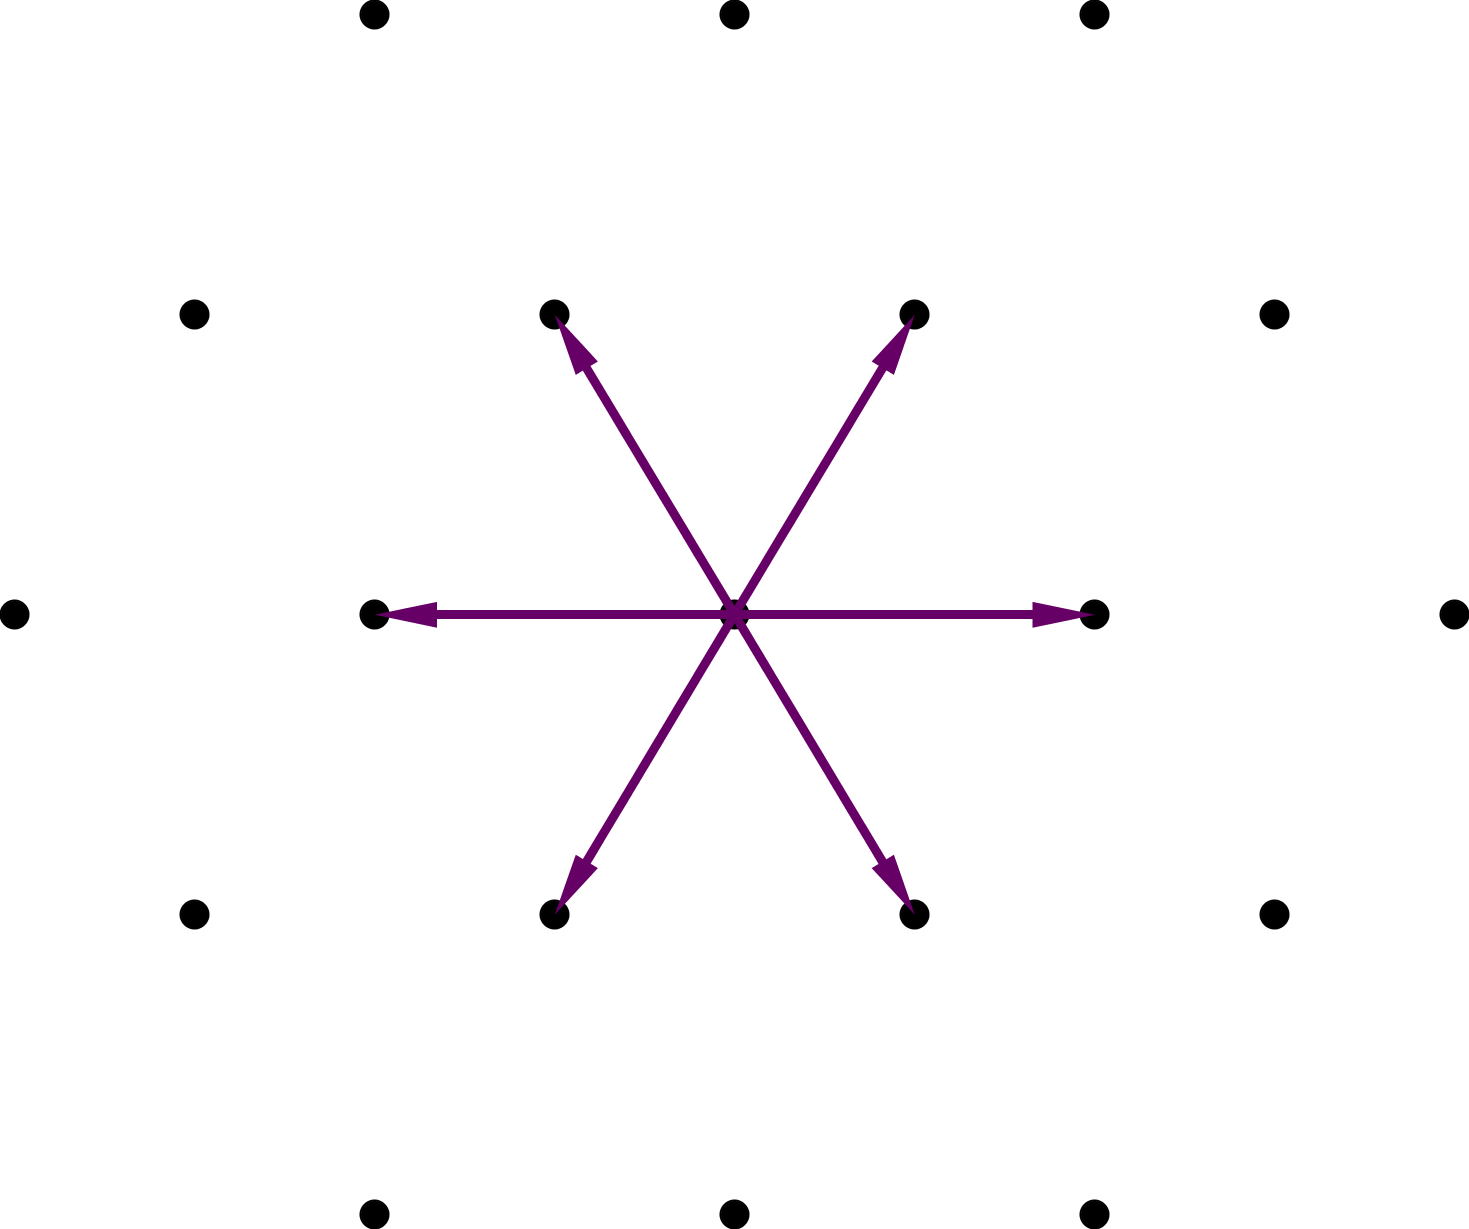
\includegraphics[width=0.6\textwidth]{./img/fhp_desc}
\end{figure}

Therefore, every node consists of the six cells corresponding to these six lattice vectors. Each of these cells can be occupied by a particle, and we identify velocities of the particles with the lattice vectors.

\section{Update rule}
In all the LGCAs that we will present, update of the lattice consists of two subsequent steps - collision and propagation.

The role of the collision is to change the state of the node as much as possible, so that viscosity is minimized.
The only constraint on the collision rule is to preserve the number of particles (conservation of mass) and to preserve the total momentum in the node (conservation of momentum).

These requirements lead only to a handful of collision configurations, see figure \ref{FHPcol}. For the simplicity, we are considering the FHP-I model, that does not included the "rest particles", otherwise we would have to include few more collisions.

\begin{figure}[H]
 \centering
 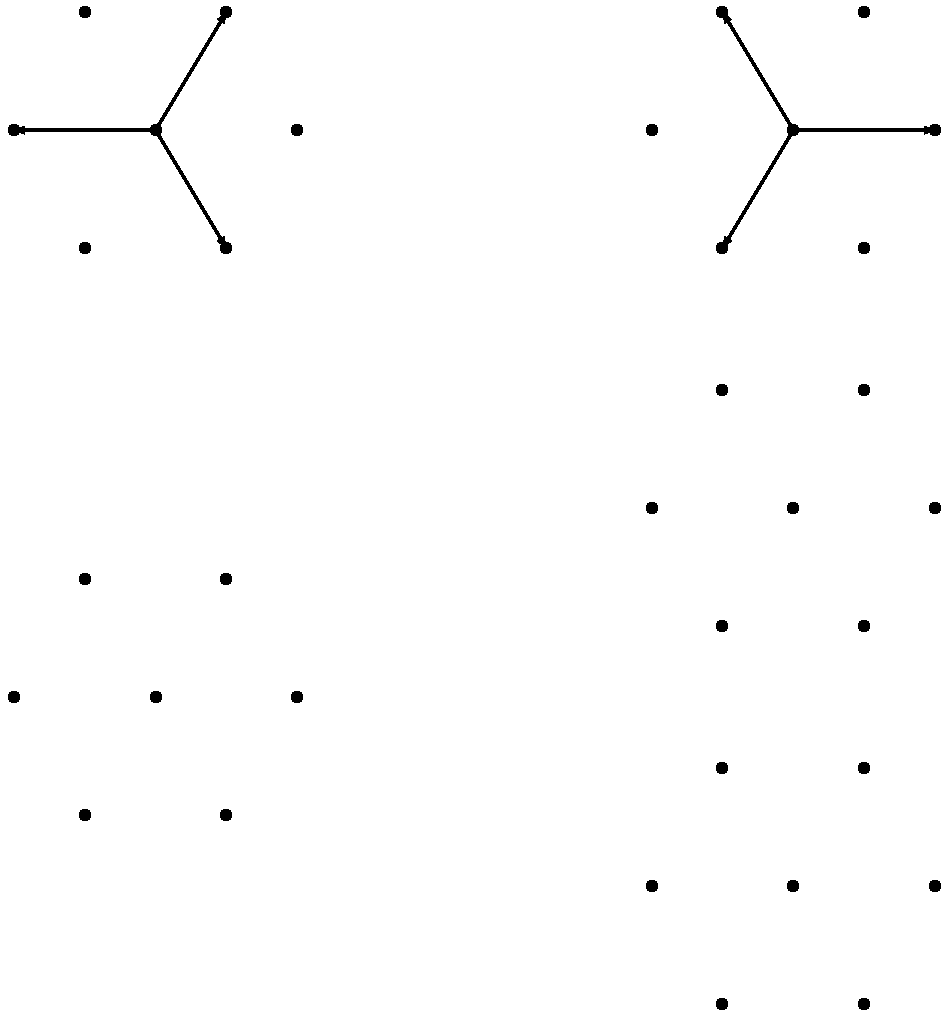
\includegraphics[width=0.7\textwidth]{./img/FHPcol}
 \caption{FHP collisions without rest particle.}
 \label{FHPcol}
\end{figure}

We see that two and four particle configurations can be resolved in two different configurations. The resulting state need to be chosen randomly, with probability $1/2$ for each state (if there was a preferred configuration, the model would posses a non-physical invariant -- chirality).

When the collision is resolved in every node, propagation follows.
This phase is straigt-forward -- if the cell is occupied by a particle, it propagates along the corresponding lattice vector to the neighboring node, see figure \ref{FHPprop}.


\begin{figure}[H]
 \centering
 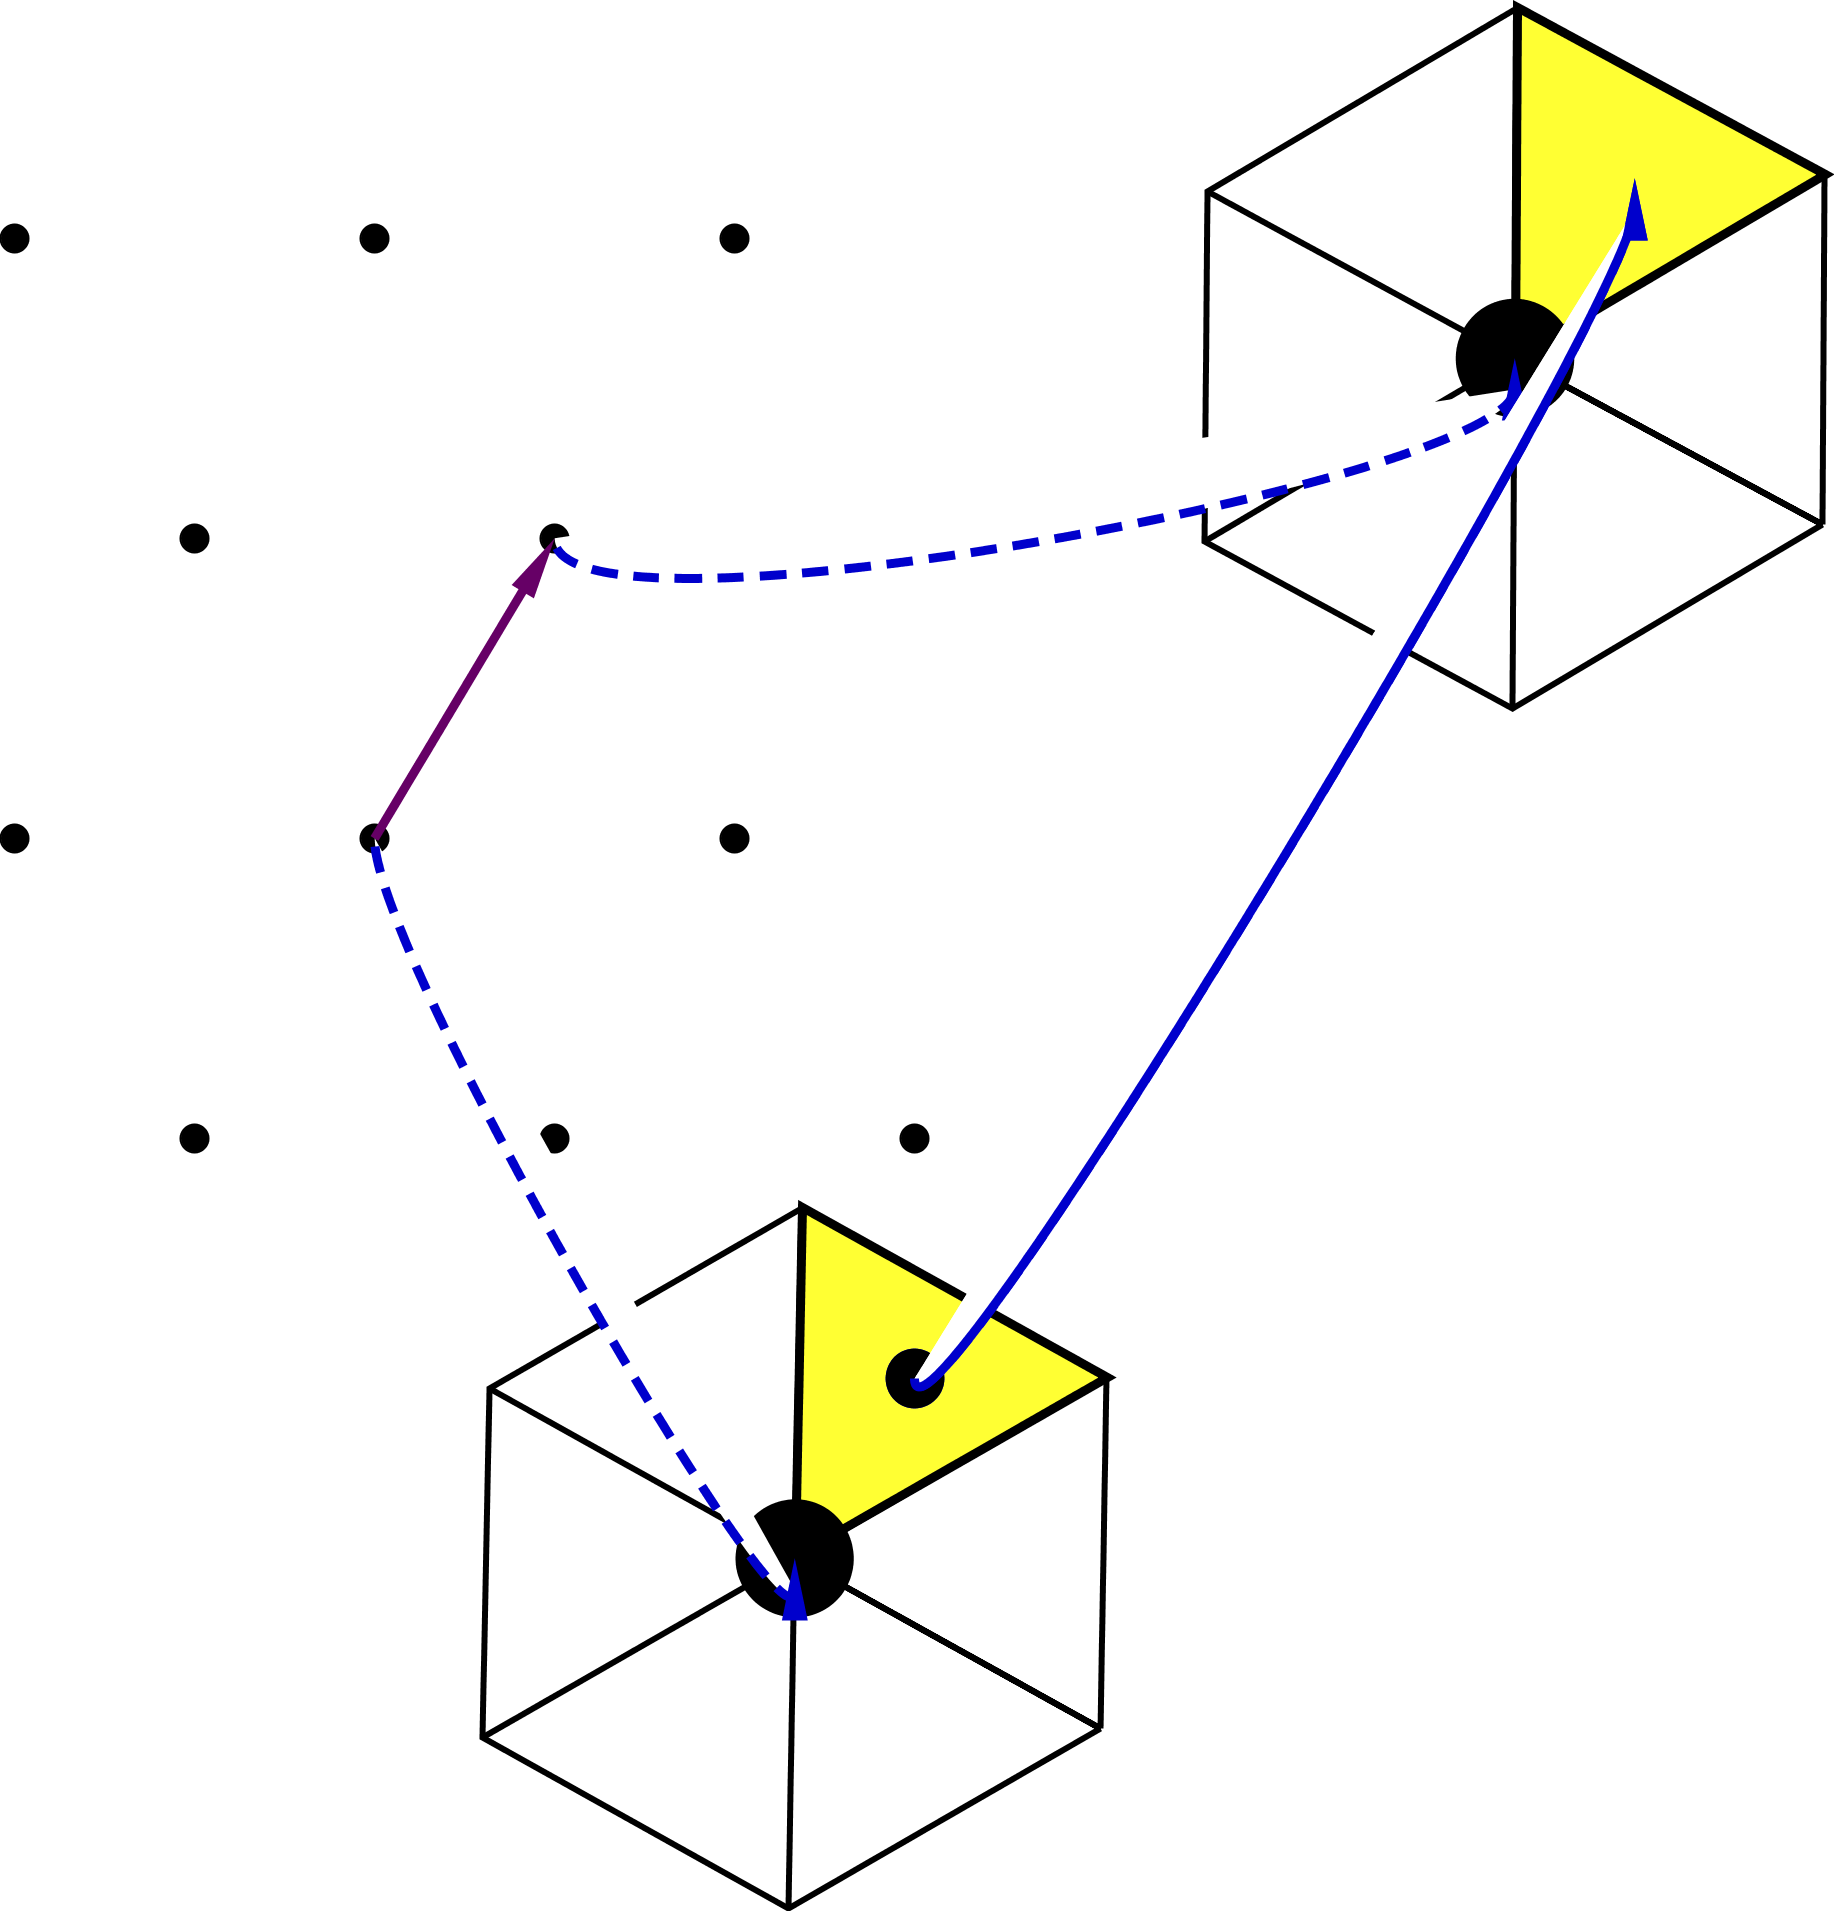
\includegraphics[width=0.7\textwidth]{./img/FHPprop}
 \caption{FHP collisions without rest particle.}
 \label{FHPprop}
\end{figure}

Comparing it to HPP, we have a mesh with better rotational symmetry and nodes with richer  set of collisions.

Now that we presented the setting of FHP in two dimensions, let us explore the microdynamics of FHP in more formal way. This formal treatment enables us to derive the hydrodynamic equations for FHP-like automata in arbitrary dimension (although finding an appropriate multidimensional lattice is non-trivial and possible only in 4 dimensions, as we will see).


Although we will form 
In the previous chapters, we seen how FHP and HPP works in intuitive way. 
In this chapter, we will treat this automata more analytically, hence we need to get more formal.

We will try to make this chapter more general, so that the obtained statistical limit is applicable for all cellular automata from the same class as FHP - specifically its predecessor HPP and its 3D upgrade FCHC.

\bigskip

But since we already have concrete idea of how FHP works, it will be the good point to start.

\section{FHP analytically}

Now that we have good intuition about FHP model, we need to get more formal to treat LGCA analytically.

State of the node will be denoted by $n = (n_1,n_2,n_3,n_4,n_5,n_6)$, where $n_i = 0$ means that $i^{th}$ cell in the node is empty, and $n_i = 1$ means that there is particle in the $i^{th}$ cell.

State of the \textbf{specific node} (at the position \textbf{r} on the lattice) will be denoted by $\bf{n(r)}$, whereas state of \textbf{all the nodes} in the lattice will be denoted by \textbf{n(.)}.

We already know that update of the whole lattice is local, hence we can treat it node by node.

We also know that update happens in discrete time steps, and it can be divided into two sub-steps - collision, and propagation.

\section{Propagation}
Propagation is straight-forward for all types of LGCA and can be captured by very simple equation
\begin{equation}
S n_i(\bf{r}) = n_i(\bf{r + c_i}). 
\end{equation}
This equation means that state of the $i^{th}$ cell in node \textbf{n(r)} propagates along the lattice vector $c_i$ to the neighboring node $\bf{n(r + c_i)}$, see figure below.\\
\\
To put it in the nutshell, propagation is completely determined by the geometry of the lattice. Once we know what the lattice vectors $c_i$ are, we know all about propagation (equation blabla).\\
\\
Where the dark magic of LGCAs hides is the collision step.\\

\section{Collision}
The purpose of collision is to change the configuration of the node as much as possible (it means to change as many bits of the node as possible), while we preserve mass and momentum.\\
(if we change direction of the particle). 

For HPP, we have only $2^4 = 16$ possible states in node, and only two collision configurations among them. Since these configurations are symmetric, we have only one collision rule.\\
For FHP, we have $2^6 = 64$ configurations, and whole bunch of collision configurations among them, but we can still draw the simple picture of these configurations:\\
\\
As we see, head-on 2-particle collisions can result in two different states. If we wanted to preserve determinism, and we were systematically choosing only one of them, we would introduce additional, non-physical invariance - the model would become chiral. If we want to preserve the parity symmetry of the model, we need to assign equal probability to either of two final states.Hence, we are introducing non-determinism to the model.

We will express the probabilities of transition from state $n$ to state $n'$ by probability matrix:
\begin{equation}
A(n \rightarrow n') \geq 0
\end{equation}
As we have 64 possible states of the node, matrix A is of dimension $64\times 64$.
For example, the cell of matrix A that governs the head-on collisions looks like this:
\[
 A'=
  \begin{bmatrix}
    0 & \frac{1}{2} & \frac{1}{2} \\
    \frac{1}{2} & 0 & \frac{1}{2} \\
    \frac{1}{2} & \frac{1}{2} & 0 \\
  \end{bmatrix}
\]
Since the collisions are symmetric, matrix A is symmetric as well.

Also, collisions are invariant to rotations or reflections of the node:
\begin{equation}
A(g(n) \rightarrow g(n')) = A(n \rightarrow n')
\end{equation}
where $g \in G$, and G is the symmetry group of the node.

\section{Collision operator}
Interestingly, we can express the whole update step in one simple equation using collision operator $\Delta_i$:
\begin{equation}
n_i(t+1,r+c_i) = n_i(t,r) + \Delta_i(t,r)
\end{equation}
If this equation works, then, $\Delta_i$ must be:
\begin{enumerate}
\item $\Delta_i = 0$ if no collision is happening in $n(t,r)$. Then state of the cell $n_i(t,r)$ only propagates to $n_i(t+1,r+c_i)$.
\item $\Delta_i = 1$ if there is not particle in $n_i(t,r)$ yet, but gets there after collision. 
 \item $\Delta_i = -1$ if there is particle in the $n_i(t,r)$, but after collision, cell gets empty.
\end{enumerate}

\bigskip

For example, $\Delta_i$ acquire very simple form for HPP:
\begin{equation}
\Delta_i = n_{i+1} n_{i+3}( 1 - n_i)(1 - n_{i+2}) - n_i n_{i+2}(1-n_{i+1})(1 - n_{i+3})
\end{equation}
As there are only 2 collision configuration in HPP, $\Delta_i$ has 2 terms.
If either collision happens, corresponding term is 1.

\section{Microscopic conservation laws}
Using collision operator, conservation of mass and momentum is this simple:
\begin{subequations}
\begin{align}
\sum_i \Delta_i(t,r) &= 0,\\
%
\sum_i c_i \Delta_i(t,r) &= 0
\end{align}
\end{subequations}
(Prove: unfold $\Delta$s)
Conservation laws can be equivalently expressed in the form
\begin{align} \label{cons1}
\begin{split}
\sum_i n_i(t+1, r + c_i) &= \sum_i n_i(t,r), \\
\sum_i c_i n_i(t+1, r + c_i) &= \sum_i c_i n_i(t,r).
\end{split}
\end{align}